\centering
\usetikzlibrary{arrows, shapes, calc, fit, shapes.geometric}
\definecolor{mygreen}{rgb}{0.00,0.5,0.00}
\definecolor{myblue}{rgb}{0,0,0.6}
\definecolor{myred}{rgb}{1,0,0}
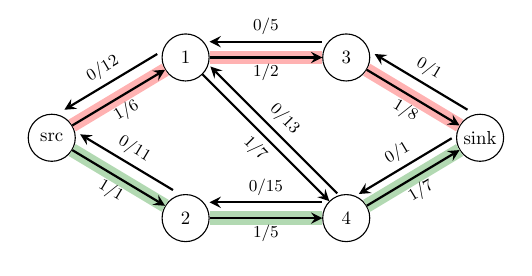
\begin{tikzpicture}[scale=0.68]
\tikzset{VertexStyle/.style =
    {draw, shape=circle,minimum size=25pt,inner sep=0pt, scale=0.68}
}
\tikzset{PredStyle/.style = {transform canvas={xshift=1.5mm, yshift=1.5mm}, text=mygreen}}
\tikzset{LabelStyle/.style = {text=black, font=\small, below, scale=0.8, sloped}}
\tikzset{SelectedEdgeStyle/.style = {draw, line width=5pt, mygreen!30}}
\tikzset{EdgeStyle/.style = {->, thick, -stealth}}
\tikzset{LabelStyle/.style = {text=black, font=\small, below, scale=0.67, sloped}}
\begin{scope}[scale=1.0, every node/.style={scale=1.0}, every edge/.style={scale=1.2}]
\node[VertexStyle] (G-res-src) at (-4,0) {src};
\node[VertexStyle] (G-res-sink) at (4,0) {sink};
\foreach \index/\name in {1/1, 2/2}
    \node[VertexStyle] (G-res-\name) at (-1.5,{3*(1.5-\index)}) {$\name$};
\foreach \index/\name in {1/3, 2/4}
    \node[VertexStyle] (G-res-\name) at (1.5,{3*(1.5-\index)}) {$\name$};
\end{scope}
\tikzset{SelectedEdgeStyle/.style = {draw, line width=5pt, myred!30}}
\draw[SelectedEdgeStyle] (G-res-src) to (G-res-1);
\draw[SelectedEdgeStyle] (G-res-1) to (G-res-3);
\draw[SelectedEdgeStyle] (G-res-3) to (G-res-sink);
\tikzset{SelectedEdgeStyle/.style = {draw, line width=5pt, mygreen!30}}
\draw[SelectedEdgeStyle] (G-res-src) to (G-res-2);
\draw[SelectedEdgeStyle] (G-res-2) to (G-res-4);
\draw[SelectedEdgeStyle] (G-res-4) to (G-res-sink);
\draw[EdgeStyle] (G-res-src) to node[LabelStyle]{1/6} (G-res-1);
\draw[EdgeStyle] (G-res-src) to node[LabelStyle]{1/1} (G-res-2);
\draw[EdgeStyle] (G-res-1) to node[LabelStyle]{1/2} (G-res-3);
\draw[EdgeStyle] (G-res-2) to node[LabelStyle]{1/5} (G-res-4);
\draw[EdgeStyle] (G-res-1) to node[LabelStyle]{1/7} (G-res-4);
\draw[EdgeStyle] (G-res-3) to node[LabelStyle]{1/8} (G-res-sink);
\draw[EdgeStyle] (G-res-4) to node[LabelStyle]{1/7} (G-res-sink);

\tikzset{LabelStyle/.style = {text=black, font=\small, above, scale=0.67, sloped}}
\tikzset{EdgeStyle/.style = {<-, thick, stealth-}}
\draw[EdgeStyle, transform canvas={xshift=-1mm, yshift=2mm}] (G-res-src) to node[LabelStyle]{0/12} (G-res-1);
\draw[EdgeStyle, transform canvas={xshift=1mm, yshift=2mm}] (G-res-src) to node[LabelStyle]{0/11} (G-res-2);
\draw[EdgeStyle, transform canvas={yshift=2mm}] (G-res-1) to node[LabelStyle]{0/5} (G-res-3);
\draw[EdgeStyle, transform canvas={yshift=2mm}] (G-res-2) to node[LabelStyle]{0/15} (G-res-4);
\draw[EdgeStyle, transform canvas={xshift=1mm, yshift=1mm}] (G-res-1) to node[LabelStyle]{0/13} (G-res-4);
\draw[EdgeStyle, transform canvas={xshift=1mm, yshift=2mm}] (G-res-3) to node[LabelStyle]{0/1} (G-res-sink);
\draw[EdgeStyle, transform canvas={xshift=-1mm, yshift=1.5mm}] (G-res-4) to node[LabelStyle]{0/1} (G-res-sink);
\end{tikzpicture}
